
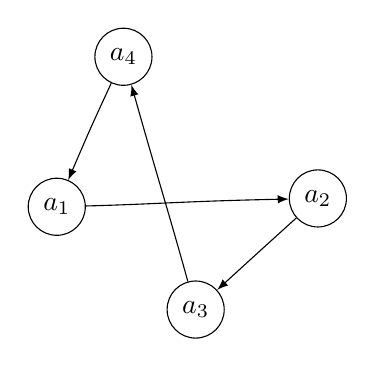
\begin{tikzpicture}[>=latex,line join=bevel,]
%%
\node (a_4) at (53bp,120bp) [draw,circle] {$a_4$};
  \node (a_3) at (79bp,29bp) [draw,circle] {$a_3$};
  \node (a_2) at (123bp,69bp) [draw,circle] {$a_2$};
  \node (a_1) at (29bp,66bp) [draw,circle] {$a_1$};
  \draw [->] (a_2) ..controls (102bp,50bp) and (102bp,50bp)  .. (a_3);
  \draw [->] (a_3) ..controls (69bp,65bp) and (66bp,74bp)  .. (a_4);
  \draw [->] (a_1) ..controls (66bp,67bp) and (75bp,68bp)  .. (a_2);
  \draw [->] (a_4) ..controls (41bp,94bp) and (41bp,94bp)  .. (a_1);
%
\end{tikzpicture}
